\chapter{Neutrino Physics}
\label{chap:theory}
\section{The Discoveries of the Neutrinos}
Neutrinos were initially proposed as a solution to the apparent violation of the conservation of four and angular momentum in James Chadwick measurements of the beta decay in 1932\cite{Chadwick1,Chadwick2}. Inspired by Wolfgang Pauli's new elementary particle ``the neutron'' (which had characteristics of what we today call a nucleon and a neutrino)\cite{pauli_1933}, Enrico Fermi built his theory of $\beta$-decay\cite{fermi_1934}, in which the observable process $n \rightarrow p + e^-$ is always accompanied by an invisible four-momentum carrier, the electron anti-neutrino.

The neutrino remained elusive until Reines and Cowan devised experiments\cite{reines_cowan_1,reines_cowan_2} in 1953, using the inverse beta decay (IBD) process, $\bar{\nu}_e + p \rightarrow n + e^+$, near a nuclear reactor. The experiment consistent of two tanks of water (100 L fiducial mass), sandwiched by liquid scintillator tanks with PMTs. The water was doped with 40 kg $\text{CdCl}_2$, which could detect free neutrons through capture. The electron anti-neutrinos were emitted by the nuclear reactor, interacted with the protons in the water, producing a prompt signal from $e^+ + e^- \rightarrow 2\gamma$. The free neutron was detected $\sim5\mu\text{s}$ after the prompt $2\gamma$ from $n + ^{108}\text{Cd} \rightarrow ^{109m}\text{Cd} \rightarrow ^{109}\text{Cd} + \gamma$. The experiment also took data from a reactor off period, demonstrating a significant reduction in neutrino event rates. The experiment was complemented by measurements by R. Davis\cite{davis} in 1964, which exposed tanks of $^{37}\text{Cl}$ to reactor electron anti-neutrinos, interacting through $\bar{\nu}_e + ^{37}\text{Cl} \rightarrow e^- + ^{37}\text{Ar}$, which would violate lepton number conservation. The experiment found no excess of $^{37}\text{Ar}$, and instead set limits on the solar neutrino flux.

The field quickly developed, and in 1962 Lederman, Schwartz, Steinberger and others\cite{lederman} observed another flavour of neutrino, the muon neutrino. They used a beam of protons impinging a target, creating a $\pi$ dominated beam which decayed following $\pi^+ \rightarrow \mu^+ + \nu_\mu$, and looked for subsequent interactions of the $\nu_\mu$ in a 10 tonne shielded aluminium spark chamber. The experiment was later confirmed by measurements at CERN in 1964\cite{cern_spark,cern_spark2}.

When the third charged lepton, the $\tau$, was discovered at SLAC's $e^+e^-$ accelerator in 1975\cite{tau_disc}, the search for its neutrino partner started. Its existence was already hinted at in $\tau$ decays, but was ultimately discovered at DONUT\cite{tau_nu_disc} in 2000. The discovery of the $\nu_\tau$ and the three neutrino flavours was confirmed by $Z \rightarrow l^+ l^-$ decays at LEP and SLAC\cite{lep}, which found the number of active neutrino flavours, assuming the Standard Model, as $N_\nu = 2.9840\pm0.0082$. This has also been confirmed by cosmological data from Planck and others\cite{planck}, $N_\text{eff} = 3.04\pm0.18$\footnote{$N_\text{eff}=3.0\pm0.4$ and $\sum m_\nu < 0.22 \text{ eV}$ when varying both $N_\text{eff}$ and $\sum m_\nu$.}.

\section{Neutrino Oscillations}
\label{sec:theory:osc}
This thesis could largely proceed without mentioning neutrino oscillations, Two-flavour model, See-saw model?

\section{Neutrino Interactions}
\label{sec:theory:int}
Invoking ideas from electron scattering

\section{Experimental Overview}
Neutrino oscillations is today an established physics phenomena, cemented by Kajita-san and Art McDonald receiving the Nobel Prize in Physics in 2015. This section briefly introduce neutrino oscillation experiments and gives an overview

\subsection{Solar Neutrinos}
Solar neutrinos emanate from various nuclear fusion products and decays in the sun. \autoref{tab:solar_flux} shows the fluxes for various sources, where clearly the $pp$ flux is strongest. However, the neutrino energy is often below threshold for the largest contributors to the flux, and most solar neutrino experiments measure the $^{8}\text{B}$ flux, shown in \autoref{fig:solar_flux}.
\begin{table}[h]
	\begin{tabular}{l | c c}
		\hline
		\hline
		Reaction & Label & Flux ($\text{cm}^{-2} \text{s}^{-1}$) \\
		\hline
		$p+p\rightarrow ^{2}\text{H} + e^+ + \nu_e$ & $pp$ & $5.95\times10^{10}$ \\
		$p+e^-+p\rightarrow ^{2}\text{H} \nu_e$ & $pep$ & $1.40\times10^{8}$ \\
		$^{3}\text{He} + p\rightarrow ^{4}\text{H} + e^+ + \nu_e$ & $hep$ & $9.3\times10^{3}$ \\
		$^{7}\text{Be} + e^- \rightarrow ^{7}\text{Li} + \nu_e$ & $^{7}\text{Be}$ & $4.77\times10^{9}$ \\
		$^{8}\text{B} \rightarrow ^{8}\text{Be}* + e^+ \nu_e$ & $^{8}\text{B}$ & $5.05\times10^{6}$ \\
		\hline
		\hline
	\end{tabular}
	\caption{Integrated solar neutrino flux from various solar processes in the $pp$ chain. Table replicated from \cite{solar_review}.}
	\label{tab:solar_flux}
\end{table}

\begin{figure}[h]
	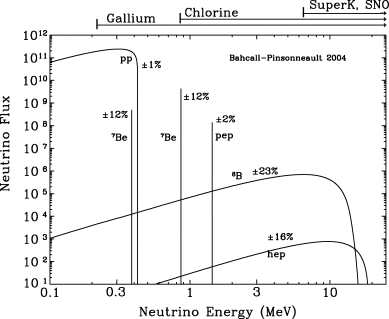
\includegraphics[width=0.5\textwidth, trim={0mm 0mm 0mm 0mm}, clip,page=1]{figures/theory/solar_flux}
	\caption{Solar flux from different $pp$ chain fusion sources, including thresholds of experiments. Figure from \cite{sno_solar_flux}.}
	\label{fig:solar_flux}
\end{figure}

R. Davis and J. Bachall would continue measurements of the solar neutrinos from $^{8}\text{B}$ and in 1968\cite{davis_sun} announced a solar $\nu_e$ flux a factor seven of expected ($\sim2\sigma$ significance), largely attributed to solar model calculations. This was the birth of the ``solar neutrino problem'', which Bruno Pontecorvo and Vladimir Gribov in 1969\cite{pontecorvo_gribov} proposed a solution to by invoking a $\nu_e\leftrightarrow\nu_\mu$ oscillation similar to $K^0 \leftrightarrow\bar{K}^0$. In 1989, the Kamiokande experiment\cite{kamiokande_solar} confirmed the result, measuring a $^{8}\text{B}$ solar neutrino flux of $\sim0.5$ the expected, agreeing with the higher statistic data from Homestake\cite{davis_sun2}. The solar neutrino deficit was confirmed from the low threshold detectors SAGE\cite{sage_solar} and GALLEX\cite{gallex_solar}, additionally capable of detecting $p p$ neutrinos using $^{71}\text{Ga}+\nu_e \rightarrow ^{71}\text{Ge}+e^-$.

The Sudbury Neutrino Observatory (SNO) put the nail in the coffin in 2002\cite{sno_solar} by measuring the solar $\nu$ from $^{8}\text{B}$ in three channels: $\nu_e + d \rightarrow p+p+e^-$ (CC), $\nu_x + d\rightarrow p+ n + \nu_x$ (NC) and $\nu_x + e^- \rightarrow \nu_x+e^-$ (ES). The measured fluxes had a $\nu_e$ component consistent with previous measurements, a strong non-$\nu_e$ component 5.3$\sigma$ above zero, and a NC component consistent with predictions from solar models.

Additionally, the low threshold, low background, Borexino experiment has detected solar neutrinos from the $^{8}\text{B}$, $^{7}\text{Be}$, $pep$, CNO and $pp$ processes\cite{borexino_summary}. The next-generation SNO experiment, SNO+, aims to confirm and improve these measurements, and make detailed measurements of the MSW effect, solar metallicty and luminosity.

Although the solar neutrino oscillation parameters $\Delta m^2_{21}$ and $\theta_{21}$ are considered well-constrained, there is $\sim 2\sigma$ tension on $\Delta m^2_{21}$ between SK+SNO (which are compatible), and the reactor anti-neutrino experiment, KamLAND\cite{m2_tension}.

\subsection{Atmospheric Neutrinos}
Atmospheric neutrinos are emitted when cosmic rays interact with nuclei in the earth's atmosphere, producing mesons which decay into neutrinos, amongst others. The primary decay is the pion decay,
\begin{gather*}
	\pi^\pm \rightarrow \mu^\pm + \nu_\mu(\bar{\nu}_\mu) \\
	\mu^\pm \rightarrow e^\pm + \bar{\nu}_\mu (\nu_\mu) + \nu_e (\bar{\nu}_e)
\end{gather*}
giving rise to a total of three neutrinos. The neutrino flux from Honda\cite{honda_flux} is shown in \autoref{fig:atmos_flux}, which peaks in the 1-100 GeV region, notably higher than the solar neutrinos.
\begin{figure}[h]
	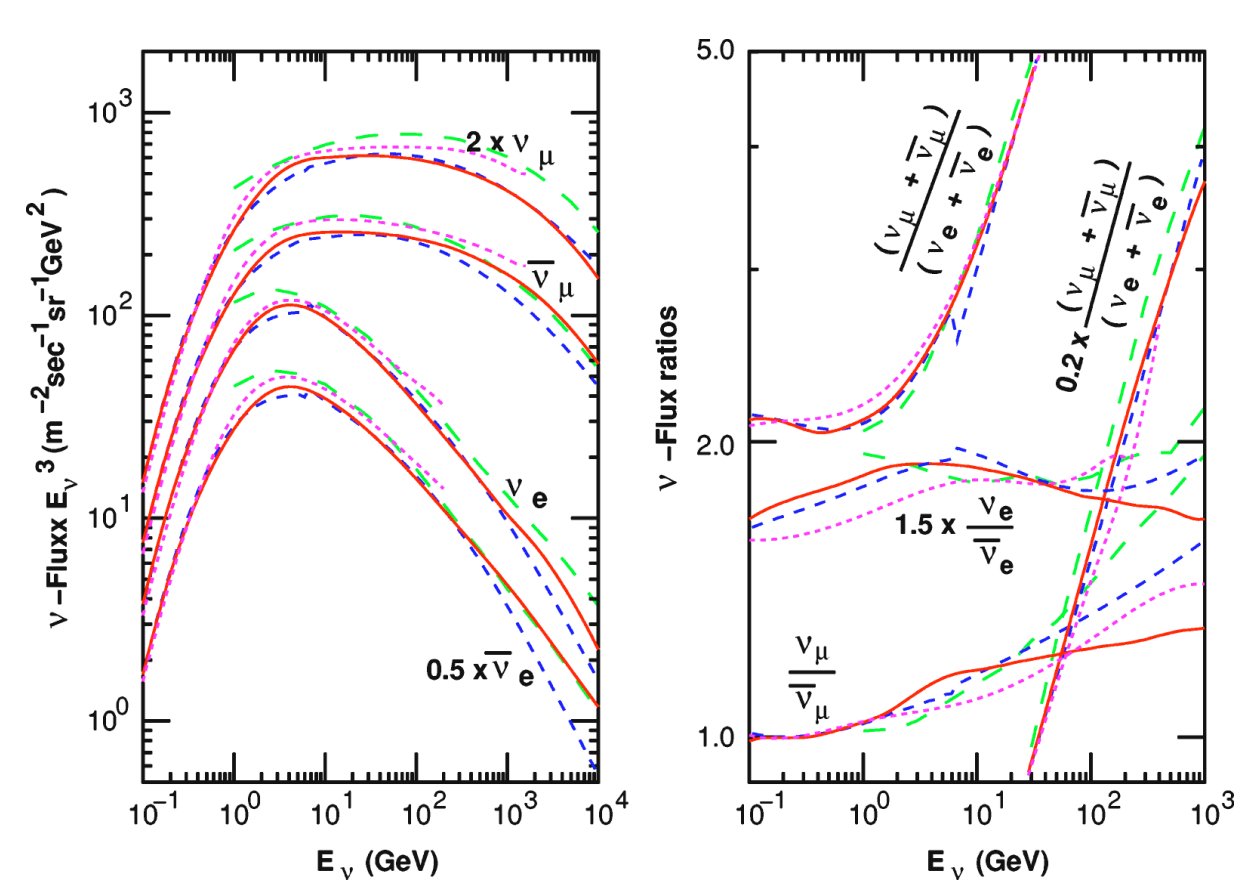
\includegraphics[width=0.7\textwidth, trim={0mm 0mm 0mm 0mm}, clip,page=1]{figures/theory/honda_flux}
	\caption{Atmospheric neutrino flux from \cite{honda_flux}.}
	\label{fig:atmos_flux}
\end{figure}

In 1965 F. Reines\cite{reines_atmos} and C.V. Achar\cite{india_atmos_hint} first saw hints of atmospheric $\nu_\mu$ appearance in deep underground laboratories through $\nu_\mu(\bar{\nu}_\mu) + X \rightarrow \mu^\pm + X'$. The Irvine-Michigan-Brookhaven (IMB) experiment\cite{imb} observed deficits of $\nu_\mu$ in 1986, and Kamiokande II in 1988\cite{kamiokande_atmos_hint} verified this and found muon-like events of $59\pm7\%$ the prediction, although good agreement of electron-like single-prong events. The Soudan-2 experiment\cite{soudan2} also saw indications of muon neutrino deficiency, seeing a neutrino flavour ratio of $0.72\pm0.19^{+0.05}_{-0.07}$ relative expectation. 

When Super-Kamiokande in 1998 published\cite{sk_disc} their high-statistics (4353 fully-contained+301 partially-contained) $\nu_\mu$ data, they found $R=\left( \mu/e \right)_\text{Data}/\left( \mu/e \right)_\text{MC} =0.65\pm0.05\pm0.08$. They additionally fitted the oscillation parameters, finding the data was well described by $\nu_\mu \leftrightarrow \nu_\tau$ rather than $\nu_\mu \leftrightarrow \nu_e$. The summary of atmospheric $\nu$ flavour ratios is seen in \autoref{fig:atmos_ratio}, where the majority of the high precision data sits at $R=0.6-0.8$.
\begin{figure}[h]
	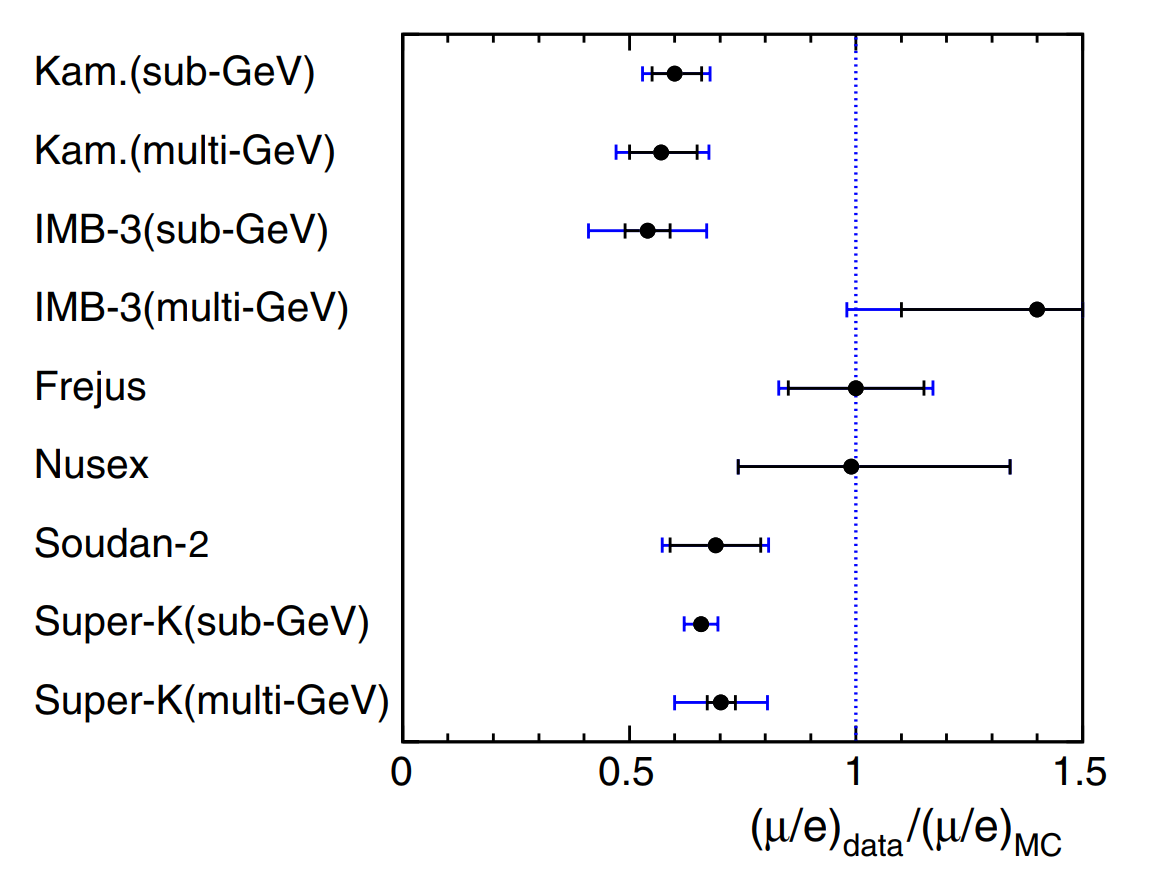
\includegraphics[width=0.7\textwidth, trim={0mm 0mm 0mm 0mm}, clip,page=1]{figures/theory/flavour_ratio}
	\caption{Measured flavour ratios for various atmospheric neutrino experiments. Figure from \cite{kajita_summary}.}
	\label{fig:atmos_ratio}
\end{figure}

Atmospheric neutrino observatories after the mid 2000s have focussed on measuring the $\nu_\mu\rightarrow\nu_\mu$ to increasing precision. Furthermore, by isolating regions of specific zenith angle (and so baseline $L$), the extent of the matter effects are also studied, which may resolve the ordering of the mass states. This is largely the focus of IceCube\cite{icecube}, ANTARES\cite{antares}, SNO+ and Super-Kamiokande's atmospheric neutrino programme. Super-Kamiokande has also made attempts at isolating $\nu_\tau$ events\cite{superk_tau}, claiming $4.6\sigma$ discovery of $\nu_\tau$ appearance in 2017. Recent results can be seen in \autoref{fig:atmos_data}.
\begin{figure}[h]
	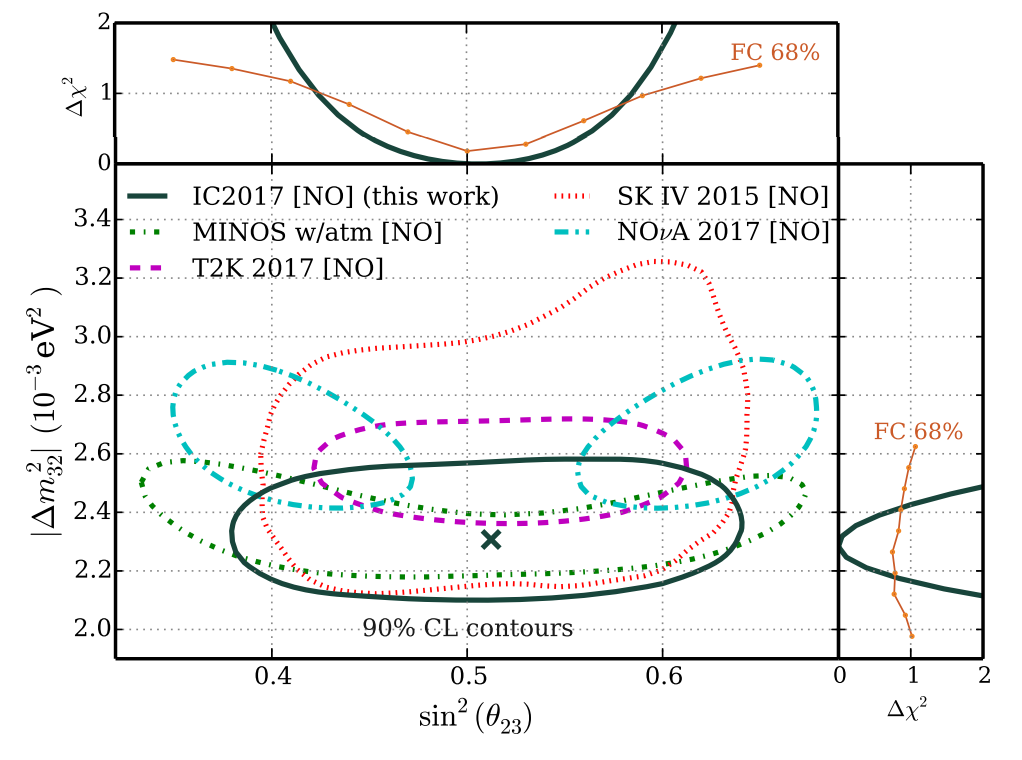
\includegraphics[width=0.7\textwidth, trim={0mm 0mm 0mm 0mm}, clip,page=1]{figures/theory/icecube_comp}
	\caption{Measured atmospheric oscillation parameters from recent atmospheric and long baseline accelerator neutrino experiments, assuming normal ordering. Figure from \cite{icecube}.}
	\label{fig:atmos_data}
\end{figure}

\subsection{Accelerator Neutrinos}
Accelerator neutrinos are similar to atmospheric neutrinos in energy, baseline and production mechanism. The neutrinos are made by impinging protons from accelerators on targets, producing a flurry of mesons which decay into neutrinos, amongst others. Experiments often have the ability to deflect and/or focus mesons after the target, enabling sign and thus $\nu_\mu$ vs $\bar{\nu_\mu}$ selection. In contrast to atmospheric, accelerator neutrinos are primarily ($\sim90\%$) muon flavoured.

The driver behind the accelerator programme was initially the atmospheric neutrino oscillations outlined above. Since the neutrino energy can be tuned in an accelerator, the oscillation dip is bombarded by statistics. Furthermore, the dependence on the atmospheric flux simulation is removed\cite{lbnl_review}. The disadvantage is the reduced total flux at the far-detector, generally forcing the baseline to $L<1000\text{ km}$ which limits the impact of the matter effect. The majority of long baseline accelerator neutrino experiments include a near detector which samples the beam before any long baseline oscillations have taken place.

The short-baseline ($L\sim 1\text{ km}$) accelerator neutrino experiments, such as MiniBooNE\cite{mb_design}, MINER$\nu$A\cite{minerva_design}, and the upcoming SBND programme\cite{sbnd}, are generally intended to measure neutrino interactions and perform short baseline oscillation searches. They may also serve as neutrino beam monitors for other experiments. The interaction measurements are used to inform neutrino event generators\cite{neut,genie,NuWro}, aiding in reducing systematic uncertainties for neutrino cross-section and oscillation experiments.

The pioneering long-baseline ($L\sim 100-1000\text{ km}$) experiments MINOS\cite{minos_obs} and K2K\cite{k2k_obs} confirmed the atmospheric neutrino mixing in $\nu_\mu \rightarrow \nu_\mu$, finding compatible oscillation parameters. The searches for $\nu_\mu \rightarrow \nu_e$ were not statistically significant\cite{k2k_noobs,minos_disc}, and were discovered by the next generation experiments T2K\cite{t2k_disc} and NO$\nu$A\cite{nova_disc}, with the $\bar{\nu}_\mu \rightarrow \bar{\nu}_e$ oscillation hinted at by NO$\nu$A at Neutrino 2018\cite{nova_neutrino2018}. The Japanese experiments K2K and T2K have consistently used the 50,000 tonne water Cherenkov detector Super-Kamiokande\cite{superk} as their far detector, with plastic scintillator based near-detectors and a baseline of $L\sim250\text{ km}$ and $E\sim0.5-2\text{ GeV}$. Both MINOS and NO$\nu$A use(d) purpose-built matching near and far-detectors, allowing for many detector systematics to be reduced, with $L\sim700\text{ km}$ and $E\sim2-5\text{ GeV}$.

In Europe, the OPERA\cite{opera} experiment was designed to look for the dominant $\nu_\mu \rightarrow \nu_\tau$ oscillation. The ICARUS\cite{icarus} experiment searched for $\nu_\mu\rightarrow\nu_e$ from steriles observed by LSND\cite{lsnd} and MiniBooNE\cite{miniboone_sterile}, which have been questioned in the community\cite{lsnd_refute}. The detection threshold for the charged current interaction $\nu_\tau + X \rightarrow \tau + X'$ is $E_\nu\sim 3.5\text{ GeV}$, so the neutrino beam from CERN to Gran Sasso (CNGS)\cite{cngs} was wide-band with $E_\nu = 10-25\text{ GeV}$. The $\tau$ detection required very fine granularity and OPERA used nuclear emulsions to accomplish this, and ICARUS pioneered the use of liquid argon TPCs in neutrino physics. OPERA claimed $\nu_\tau$ appearance\cite{opera_final_tau} at 6.1$\sigma$, and both OPERA and ICARUS found no evidence of sterile neutrinos\cite{icarus_lsnd,opera_lsnd}.

\subsection{Reactor Anti-Neutrinos}
Reactor neutrinos are formed in fission products in nuclear reactors, e.g. $^{231}\text{Th} \rightarrow ^{231}\text{Pa} + e^- + \bar{\nu}_e$ and $^{215}\text{Po} \rightarrow ^{211}\text{Pb} + e^- + \bar{\nu}_e$. The neutrino flux depends on the relative fission yields of the products, but generally have a similar energy to solar neutrinos, in the 1-10 MeV range, seen in \autoref{fig:reactor_flux}.
\begin{figure}[h]
	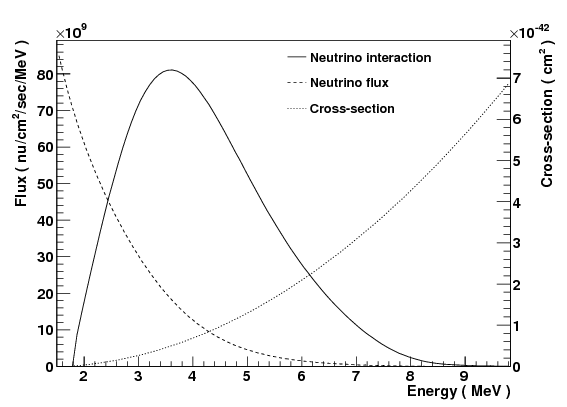
\includegraphics[width=0.4\textwidth, trim={0mm 0mm 0mm 0mm}, clip,page=1]{figures/theory/reactor_flux}
	\caption{Reactor flux for the Japanese experimental fast reactor, JOYO. Figure from \cite{reactor_flux}.}
	\label{fig:reactor_flux}
\end{figure}

They are exclusively detected by the IBD interaction, in which the $e^+ + e^- \rightarrow 2\gamma$ are measured in scintillator. Many experiments additionally dope or surround the scintillator with a high neutron capture element (e.g. $^{6}\text{Li}$ or $^{157}\text{Gd}$). In the case of Gd, this gives a prompt $2\gamma$ signal follwed by a $\sim30\mu\text{s}$ delayed $\gamma$ cascade with $E_\gamma^{tot}\sim8\text{ MeV}$, facsillitating signal-background separation. 

Similarly to accelerator neutrinos, the reactors can be split by baseline. Short baseline experiments with $L\sim1-2\text{ km}$ perform world-leading measurements of $\Delta m^2_{13}$ and $sin^2\theta_{13}$, and probing parts of the sterile neutrino spectrum. Daya Bay\cite{daya_bay_disc}, RENO\cite{reno_disc} and Double Chooz\cite{double_chooz_disc} all measured a relatively large $\sin^2 \theta_{13}$, enabling $\nu_e$ appearance to be found at long baseline neutrino experiments such as T2K and NO$\nu$A. The short baseline reactor results on $\sin^2\theta_{13}$ are often used in T2K oscillation analyses for increased sensitivity. A summary plot of the measured parameters by short baseline reactor and long baseline accelerator neutrino oscillation experiments is shown in \autoref{fig:13_sector}.
\begin{figure}[h]
	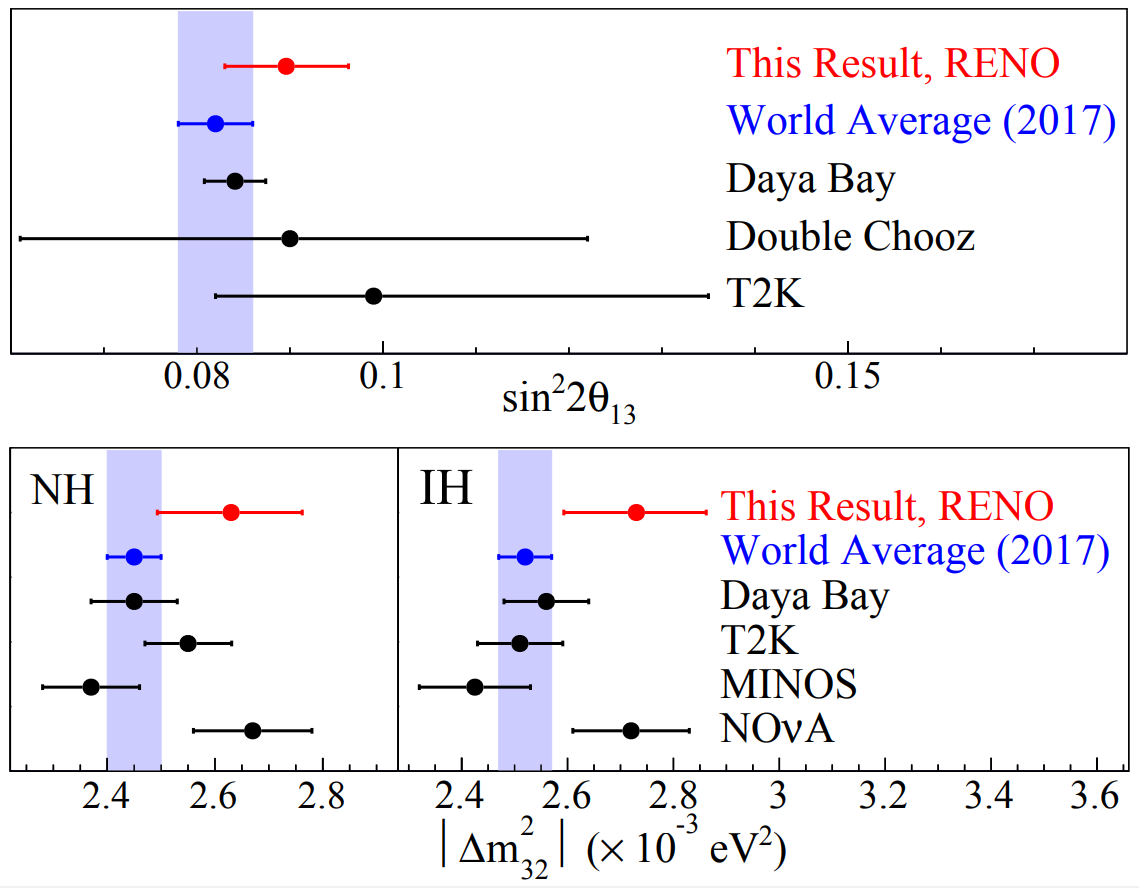
\includegraphics[width=0.5\textwidth, trim={0mm 0mm 0mm 0mm}, clip,page=1]{figures/theory/reno_theta_dm13}
	\caption{$\Delta m^2_{23}$ and $\sin^2 2\theta_{13}$ measurements from reactor (Daya Bay\cite{daya_bay}, RENO\cite{reno_new} and Double Chooz\cite{double_chooz_old}) and accelerator (T2K\cite{t2k_2015}, NO$\nu$A\cite{nova_2017} and MINOS\cite{minos_numu_nue}) neutrinos. Figure from \cite{reno_new}.}
	\label{fig:13_sector}
\end{figure}

The only medium baseline ($L\sim50\text{ km}$) under construction is JUNO\cite{juno}. The RENO collaboration has proposed\cite{reno_50} building a far detector site for RENO, equivalent to JUNO, although groundbreaking has not yet commenced. The medium baseline aims to measure the neutrino mass ordering by separating the oscillations into fast and slow parts from $\Delta m^2_{23}$ and $\Delta m^2_{12}$, and improve measurements of $\sin^2 \theta_{12}$.

KamLAND is the only long baseline $L\sim180\text{ km}$ reactor anti-neutrino experiment. It measured the $\bar{\nu}_e$ flux from 56 Japanese nuclear power reactors with good sensitivty to $\Delta m^2_{21}$, but less so to its sign due to the smaller matter effect. However, combining KamLAND with SNO and SK solar has excellent reduction on $\Delta m^2_{21}$ and $\tan^2\theta_{12}$, as shown in \autoref{fig:21_sector}. These results are used as priors in the T2K oscillation analyses.
\begin{figure}[h]
	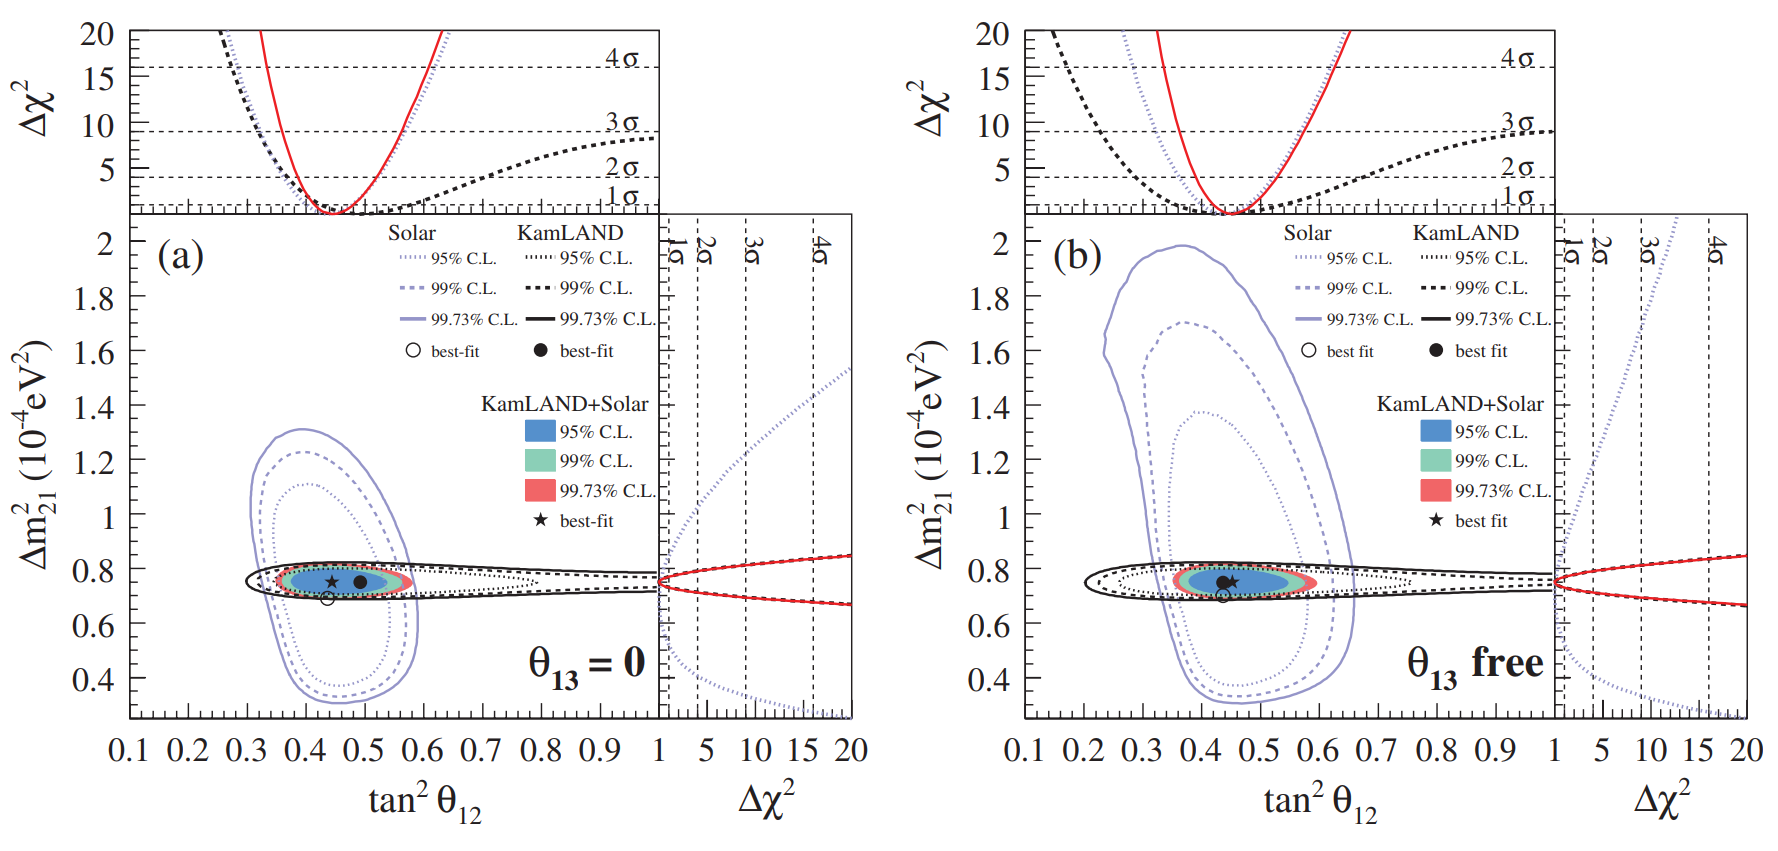
\includegraphics[width=0.7\textwidth, trim={0mm 0mm 0mm 0mm}, clip,page=1]{figures/theory/kamland_solar_comb}
	\caption{$\Delta m^2_{21}$ and $\theta_{21}$ measurements from KamLAND, SNO and Super-Kamiokande (Solar). Figure from \cite{kamland_2011}.}
	\label{fig:21_sector}
\end{figure}

Additionally, the short baseline reactors at $\sim1\text{ km}$ have measured excess at $E_\nu\sim5\text{ MeV}$\cite{double_chooz, daya_bay, reno}, which is currently unresolved. The culprit is claimed to be either poor neutrino flux modelling, or a sterile neutrino\cite{huber_neos,steriles}. As a result, very short baseline ($L\sim10-20\text{ m}$) experiments NEOS\cite{neos}, DANSS\cite{danss}, PROSPECT\cite{prospect}, STEREO\cite{stereo} and SoLi$\delta$\cite{solid} have looked for $\bar{\nu}_e$ disappearance and have not found evidence of a sterile signal and confirmed hints of a 5 MeV excess.